\documentclass{article}

% chinese fonts
\usepackage{ctex}

% math fonts
\usepackage{amsmath}
\usepackage{amsthm}
\usepackage{amssymb}
\usepackage{bm}

% figures
\usepackage{tikz}
\usepackage{graphicx}
\graphicspath{{./figures/}}

% tables
\usepackage{tabularx}
\usepackage{booktabs}
\usepackage{multirow}

% codes
\usepackage{listings}
\lstset{language     = Matlab,
        basicstyle   = \ttfamily,
        keywordstyle = \color{cyan},
        rulecolor    = \color{black},
        commentstyle = \color{green},
        keepspaces   = true,
        tabsize      = 4,
}

% hyperlinks
\usepackage{hyperref}
\hypersetup{
  breaklinks,
  colorlinks = true,
  citecolor  = blue,
  linkcolor  = red,
  urlcolor   = magenta,
}

% algorithms
\usepackage{algorithm}
\usepackage{algorithmic}

% bibliography
\usepackage[sort&compress,numbers]{natbib}

% About:  Macros for Vector, Matrix, Tensor, Math Operator and Misc
% Author: Jingxuan Yang

% vectors
\newcommand{\va}{\bm{a}}       \newcommand{\vah}{\hat{\bm{a}}}        \newcommand{\ah}{\hat{a}}    \newcommand{\vat}{\tilde{\bm{a}}}       \newcommand{\at}{\tilde{a}}
\newcommand{\vb}{\bm{b}}       \newcommand{\vbh}{\hat{\bm{b}}}        \newcommand{\bh}{\hat{b}}    \newcommand{\vbt}{\tilde{\bm{b}}}       \newcommand{\bt}{\tilde{b}}
\newcommand{\vc}{\bm{c}}       \newcommand{\vch}{\hat{\bm{c}}}        \newcommand{\ch}{\hat{c}}    \newcommand{\vct}{\tilde{\bm{c}}}       \newcommand{\ct}{\tilde{c}}
\newcommand{\vd}{\bm{d}}       \newcommand{\vdh}{\hat{\bm{d}}}        \newcommand{\dhat}{\hat{d}}  \newcommand{\vdt}{\tilde{\bm{d}}}       \newcommand{\dt}{\tilde{d}}
\newcommand{\ve}{\bm{e}}       \newcommand{\veh}{\hat{\bm{e}}}        \newcommand{\eh}{\hat{e}}    \newcommand{\vet}{\tilde{\bm{e}}}       \newcommand{\et}{\tilde{e}}
\newcommand{\vf}{\bm{f}}       \newcommand{\vfh}{\hat{\bm{f}}}        \newcommand{\fh}{\hat{f}}    \newcommand{\vft}{\tilde{\bm{f}}}       \newcommand{\ft}{\tilde{f}}
\newcommand{\vg}{\bm{g}}       \newcommand{\vgh}{\hat{\bm{g}}}        \newcommand{\gh}{\hat{g}}    \newcommand{\vgt}{\tilde{\bm{g}}}       \newcommand{\gt}{\tilde{g}}
\newcommand{\vh}{\bm{h}}     \newcommand{\vhh}{\hat{\bm{h}}}        \newcommand{\hh}{\hat{h}}    \newcommand{\vht}{\tilde{\bm{h}}}       \newcommand{\htild}{\tilde{h}}
\newcommand{\vi}{\bm{i}}       \newcommand{\vih}{\hat{\bm{i}}}        \newcommand{\ih}{\hat{i}}    \newcommand{\vit}{\tilde{\bm{i}}}       \newcommand{\itild}{\tilde{i}}
\newcommand{\vj}{\bm{j}}       \newcommand{\vjh}{\hat{\bm{j}}}        \newcommand{\jh}{\hat{j}}    \newcommand{\vjt}{\tilde{\bm{j}}}       \newcommand{\jt}{\tilde{j}}
\newcommand{\vk}{\bm{k}}       \newcommand{\vkh}{\hat{\bm{k}}}        \newcommand{\kh}{\hat{k}}    \newcommand{\vkt}{\tilde{\bm{k}}}       \newcommand{\kt}{\tilde{k}}
\newcommand{\vl}{\bm{l}}       \newcommand{\vlh}{\hat{\bm{l}}}        \newcommand{\lh}{\hat{l}}    \newcommand{\vlt}{\tilde{\bm{l}}}       \newcommand{\lt}{\tilde{l}}
\newcommand{\vm}{\bm{m}}       \newcommand{\vmh}{\hat{\bm{m}}}        \newcommand{\mh}{\hat{m}}    \newcommand{\vmt}{\tilde{\bm{m}}}       \newcommand{\mt}{\tilde{m}}
\newcommand{\vn}{\bm{n}}       \newcommand{\vnh}{\hat{\bm{n}}}        \newcommand{\nh}{\hat{n}}    \newcommand{\vnt}{\tilde{\bm{n}}}       \newcommand{\nt}{\tilde{n}}
\newcommand{\vo}{\bm{o}}       \newcommand{\voh}{\hat{\bm{o}}}        \newcommand{\oh}{\hat{o}}    \newcommand{\vot}{\tilde{\bm{o}}}       \newcommand{\ot}{\tilde{o}}
\newcommand{\vp}{\bm{p}}       \newcommand{\vph}{\hat{\bm{p}}}        \newcommand{\ph}{\hat{p}}    \newcommand{\vpt}{\tilde{\bm{p}}}       \newcommand{\pt}{\tilde{p}}
\newcommand{\vq}{\bm{q}}       \newcommand{\vqh}{\hat{\bm{q}}}        \newcommand{\qh}{\hat{q}}    \newcommand{\vqt}{\tilde{\bm{q}}}       \newcommand{\qt}{\tilde{q}}
\newcommand{\vr}{\bm{r}}       \newcommand{\vrh}{\hat{\bm{r}}}        \newcommand{\rh}{\hat{r}}    \newcommand{\vrt}{\tilde{\bm{r}}}       \newcommand{\rt}{\tilde{r}}
\newcommand{\vs}{\bm{s}}       \newcommand{\vsh}{\hat{\bm{s}}}        \newcommand{\sh}{\hat{s}}    \newcommand{\vst}{\tilde{\bm{s}}}       \newcommand{\st}{\tilde{s}}
\newcommand{\vt}{\bm{t}}       \newcommand{\vth}{\hat{\bm{t}}}        \newcommand{\that}{\hat{t}}  \newcommand{\vtt}{\tilde{\bm{t}}}       \newcommand{\ttil}{\tilde{t}}
\newcommand{\vu}{\bm{u}}       \newcommand{\vuh}{\hat{\bm{u}}}        \newcommand{\uh}{\hat{u}}    \newcommand{\vut}{\tilde{\bm{u}}}       \newcommand{\ut}{\tilde{u}}
\newcommand{\vv}{\bm{v}}       \newcommand{\vvh}{\hat{\bm{v}}}        \newcommand{\vhat}{\hat{v}}    \newcommand{\vvt}{\tilde{\bm{v}}}       \newcommand{\vtild}{\tilde{v}}
\newcommand{\vw}{\bm{w}}       \newcommand{\vwh}{\hat{\bm{w}}}        \newcommand{\wh}{\hat{w}}    \newcommand{\vwt}{\tilde{\bm{w}}}       \newcommand{\wt}{\tilde{w}}
\newcommand{\vx}{\bm{x}}       \newcommand{\vxh}{\hat{\bm{x}}}        \newcommand{\xh}{\hat{x}}    \newcommand{\vxt}{\tilde{\bm{x}}}       \newcommand{\xt}{\tilde{x}}
\newcommand{\vy}{\bm{y}}       \newcommand{\vyh}{\hat{\bm{y}}}        \newcommand{\yh}{\hat{y}}    \newcommand{\vyt}{\tilde{\bm{y}}}       \newcommand{\yt}{\tilde{y}}
\newcommand{\vz}{\bm{z}}       \newcommand{\vzh}{\hat{\bm{z}}}        \newcommand{\zh}{\hat{z}}    \newcommand{\vzt}{\tilde{\bm{z}}}       \newcommand{\zt}{\tilde{z}}

\newcommand{\valpha}{\bm{\alpha}}
\newcommand{\vbeta}{\bm{\beta}}
\newcommand{\vgamma}{\bm{\gamma}}
\newcommand{\vtheta}{\bm{\theta}}
\newcommand{\vlambda}{\bm{\lambda}}
\newcommand{\vmu}{\bm{\mu}}
\newcommand{\vomega}{\bm{\omega}}

\newcommand{\mSigma}{\bm{\Sigma}}

\newcommand{\Fc}{\mathcal{F}}
\newcommand{\Xc}{\mathcal{X}}
\newcommand{\Yc}{\mathcal{Y}}
\newcommand{\Zc}{\mathcal{Z}}
\newcommand{\Gc}{\mathcal{G}}
\newcommand{\Hc}{\mathcal{H}}
\newcommand{\Dc}{\mathcal{D}}
\newcommand{\Cc}{\mathcal{C}}
\newcommand{\Rc}{\mathcal{R}}

% matrices
\newcommand{\ma}{\bm{A}}
\newcommand{\mb}{\bm{B}}
\newcommand{\md}{\bm{D}}
\newcommand{\mH}{\bm{H}}
\newcommand{\mE}{\bm{E}}
\newcommand{\mi}{\bm{I}}
\newcommand{\mk}{\bm{K}}
\newcommand{\ml}{\bm{L}}
\newcommand{\mn}{\bm{N}}
\newcommand{\mP}{\bm{P}}
\newcommand{\mq}{\bm{Q}}
\newcommand{\mr}{\bm{R}}
\newcommand{\mU}{\bm{u}}
\newcommand{\mv}{\bm{v}}
\newcommand{\mw}{\bm{W}}
\newcommand{\mx}{\bm{X}}
\newcommand{\my}{\bm{Y}}
\newcommand{\mz}{\bm{Z}}

% tensors
\newcommand{\tp}{\mathsf{P}}
\newcommand{\tu}{\mathsf{U}}
\newcommand{\tx}{\mathsf{X}}
\newcommand{\ty}{\mathsf{Y}}
\newcommand{\tz}{\mathsf{Z}}
\newcommand{\tw}{\mathsf{W}}
\newcommand{\tf}{\mathsf{F}}
\newcommand{\ta}{\mathsf{A}}
\renewcommand{\th}{\mathsf{H}}

% norms
\newcommand{\mynorm}[2]{\| {#1} \|_{#2}}
\newcommand{\norm}[2]{\mynorm{#1}{#2}}
\newcommand{\bignorm}[2]{\left\| {#1} \right\|_{#2}}
\newcommand{\norml}[1]{\mynorm{#1}{1}}
\newcommand{\bignorml}[1]{\bignorm{#1}{1}}
\newcommand{\infnorm}[1]{\mynorm{#1}{\infty}}
\newcommand{\biginfnorm}[1]{\bignorm{#1}{\infty}}
\newcommand{\oneinf}{\ell_{1,\infty}}
\newcommand{\onetwo}{\ell_{1,2}}
\newcommand{\oneinfnorm}[1]{\mynorm{#1}{1,\infty}}
\newcommand{\bigoneinf}[1]{\bignorm{#1}{1,\infty}}
\newcommand{\onetwonorm}[1]{\mynorm{#1}{1,2}}
\newcommand{\bigonetwo}[1]{\bignorm{#1}{1,2}}
\newcommand{\enorm}[1]{\mynorm{#1}{2}}
\newcommand{\bigenorm}[1]{\bignorm{#1}{2}}
\newcommand{\znorm}[1]{\mynorm{#1}{0}}
\newcommand{\bigznorm}[1]{\bignorm{#1}{0}}
\newcommand{\frob}[1]{\|{#1}\|_{\text{F}}}
\newcommand{\bigfrob}[1]{\bignorm{#1}{\text{F}}}
\newcommand{\grpnorm}[2]{\norm{#1}{\text{Gr}(#2)}}

% math operators
\DeclareMathOperator*{\argmin}{argmin}
\DeclareMathOperator*{\argmax}{argmax}
\DeclareMathOperator{\divg}{div}
\DeclareMathOperator{\dom}{dom}
\DeclareMathOperator{\interior}{int}
\DeclareMathOperator{\ri}{ri}
\DeclareMathOperator{\sgn}{sgn}
\DeclareMathOperator{\trace}{Tr}
\DeclareMathOperator{\diag}{diag}
\DeclareMathOperator{\rank}{rank}
\DeclareMathOperator{\range}{range}
\DeclareMathOperator{\vect}{vec}
\DeclareMathOperator{\prox}{prox}
\DeclareMathOperator{\intr}{int}
\DeclareMathOperator{\relint}{ri}

% misc
\newcommand{\gs}{\geqslant}
\newcommand{\ls}{\leqslant}
\newcommand{\set}[1]{\left\{ {#1}\right\}}

\newcommand{\defeq}{\ \stackrel{\text{def}}{=}\ }
\newcommand{\ip}[2]{\left\langle#1, #2\right\rangle}
\newcommand{\reals}{\mathbb{R}}
\newcommand{\complex}{\mathbb{C}}
\newcommand{\half}{\frac{1}{2}}

\newtheorem{theorem}{Theorem}
\newtheorem{lemma}[theorem]{Lemma}
\newtheorem{proposition}[theorem]{Proposition}
\newtheorem{remark}[theorem]{Remark}
\newtheorem{corollary}[theorem]{Corollary}
\newtheorem{definition}[theorem]{Definition}


\setlength{\oddsidemargin}{-0.25 in}
\setlength{\evensidemargin}{-0.25 in} 
\setlength{\topmargin}{-0.25in} 
\setlength{\textwidth}{7 in} 
\setlength{\textheight}{8.5 in}
\setlength{\headsep}{0.25 in} 
\setlength{\parindent}{0 in}
\setlength{\parskip}{0.1 in}

\newcommand{\homework}[5]{
  \pagestyle{myheadings} 
  \thispagestyle{plain}
  \newpage
  \setcounter{page}{1} 
  \setcounter{section}{#5} 
  \noindent
  \begin{center}
    \framebox{ 
      \vbox{
        \vspace{2mm} 
        \hbox to 6.28in { {\bf
        THU-70250043-0,~Pattern~Recognition~(Spring 2021) \hfill Homework: 13} }
        \vspace{6mm} 
        \hbox to 6.28in { {\Large \hfill #1 \hfill} }
        \vspace{6mm} 
        \hbox to 6.28in { {\it Lecturer: #2 \hfill} }
        \vspace{2mm} 
        \hbox to 6.28in { {\it \hspace{14mm} #3 \hfill} }
        \vspace{2mm} 
        \hbox to 6.28in { {\it Student: #4 \hfill} }
        \vspace{2mm} 
      } 
    }
  \end{center}
  \markboth{#1}{#1} 
  \vspace*{4mm} 
}

\begin{document}

\homework{Clustering Methods}{Changshui Zhang \hspace{5mm} {\tt zcs@mail.tsinghua.edu.cn}}{Hong Zhao \hspace{16mm} {\tt vzhao@tsinghua.edu.cn}}{Jingxuan Yang \hspace{10mm} {\tt yangjx20@mails.tsinghua.edu.cn}}{8}


\section*{K-means}

1. Consider a set $D$ of $n=2k+1$ samples, $k$ of which coincide at $x=-2$, $k$ at $x=0$ and one at $x=a>0$. As you have learned in class, we are always trying to minimize the distortion measure in K-means, given by
\begin{equation}
  J_{e}=\sum_{D_{i}\neq\varnothing}\sum_{x\in D_{i}}\|x-m_{i}\|^2
\end{equation}
where $m_i$ is the mean value of the samples of the nonempty subset $D_i$.

1.1 Show that the two-cluster partitioning that minimizes $J_e$ groups the $k$ samples at $x=0$ with the one at $x=a$ if $a^2<2(k+1)$.

解: 首先证明 $k$ 个位于 $x=-2$ 的样本属于同一类. 

假设 $x_i=-2\in D_1$, $x_j=-2\in D_2$, 我们可以断言将 $x_i$ 从 $D_1$ 取出放入 $D_2$ 会使得 $J_e$ 下降, 因为如若不然则将 $x_j$ 从 $D_2$ 取出放入 $D_1$ 会使得 $J_e$ 下降. 因此, 所有 $k$ 个位于 $x=-2$ 的样本属于同一类. 同理可知 $k$ 个位于 $x=0$ 的样本也属于同一类. 所以, 在进行两类聚类时, 全部可能的结果有三种情况:

\begin{itemize}
  \item[(a)] $x=-2,x=0\in D_1$, $x=a\in D_2$
  \item[(b)] $x=-2,x=a\in D_1$, $x=0\in D_2$ 
  \item[(c)] $x=-2\in D_1$, $x=0,x=a\in D_2$
\end{itemize}

对三种情况分别计算 $J_e$ 可得
\begin{equation}
  \begin{aligned}
    J_e(a)&=k\|-2-(-1)\|^2+k\|0-(-1)\|^2=2k\\
    J_e(b)&=k\left\|-2-\frac{-2k+a}{k+1}\right\|^2+\left\|a-\frac{-2k+a}{k+1}\right\|^2=\frac{k}{k+1}(a+2)^2\\
    J_e(c)&=k\left\|0-\frac{a}{k+1}\right\|^2+\left\|a-\frac{a}{k+1}\right\|^2=\frac{k}{k+1}a^2\\
  \end{aligned}
\end{equation}

由 $a>0$ 可知 $J_e(b)>J_e(c)$, 若 $a^2<2(k+1)$, 则
\begin{equation}
  J_e(c)=\frac{k}{k+1}a^2<2k=J_e(a)
\end{equation}

因此, 当 $a^2<2(k+1)$ 时, 两类聚类的情况为 (c), 即 $k$ 个 $x=-2$ 的点属于一个类, $k$ 个 $x=0$ 的点以及 $x=a$ 属于另一个类.

1.2 What is the optimal grouping if $a^2>2(k+1)$?

解: 由 1.1 可知当 $a^2>2(k+1)$ 时, 有
\begin{equation}
  J_e(b)>J_e(c)>J_e(a)
\end{equation} 

因此两类聚类的情况为 (a), 即 $k$ 个 $x=-2$ 的点与 $k$ 个 $x=0$ 的点属于一个类, $x=a$ 属于另一个类.

\section*{Hierarchical Clustering}

2. Consider a hierarchical clustering procedure in which clusters are merged to produce the smallest increase in the sum-of-squared error at each step. If the $i$-th cluster contains $n_i$ samples with the sample mean $\vm_i$, show that the smallest increase results from merging the pair of clusters for which
\begin{equation}
  \frac{n_i n_j}{n_i+n_j}\left\|\vm_i-\vm_j\right\|^2
\end{equation}
is minimum.

解: 合并第 $i$ 类与第 $j$ 类的均方误差增量为
\begin{equation}
  \begin{aligned}
    \Delta E
    &=\sum_{\vx\in D_i,D_j}\left\|\vx-\frac{n_i\vm_i+n_j\vm_j}{n_i+n_j}\right\|^2-\sum_{\vx\in D_i}\|\vx-\vm_i\|^2-\sum_{\vx\in D_j}\|\vx-\vm_j\|^2\\
    &=\sum_{\vx\in D_i,D_j}\left[\vx^\top\vx-2\vx^\top\frac{n_i\vm_i+n_j\vm_j}{n_i+n_j}+\frac{(n_i\vm_i+n_j\vm_j)^\top(n_i\vm_i+n_j\vm_j)}{(n_i+n_j)^2}\right]\\
    &\quad-\sum_{\vx\in D_i}(\vx^\top\vx-2\vx^\top\vm_i+\vm_i^\top\vm_i)-\sum_{\vx\in D_j}(\vx^\top\vx-2\vx^\top\vm_j+\vm_j^\top\vm_j)\\
    &=-\frac{(n_i\vm_i+n_j\vm_j)^\top(n_i\vm_i+n_j\vm_j)}{n_i+n_j}+n_i\vm_i^\top\vm_i+n_j\vm_j^\top\vm_j\\
    &=-\frac{(n_i\vm_i+n_j\vm_j)^\top(n_i\vm_i+n_j\vm_j)}{n_i+n_j}+\frac{(n_i\vm_i^\top\vm_i+n_j\vm_j^\top\vm_j)(n_i+n_j)}{n_i+n_j}\\
    &=\frac{-2n_in_j\vm_i^\top\vm_j+n_in_j\vm_i^\top\vm_i+n_in_j\vm_j^\top\vm_j}{n_i+n_j}\\
    &=\frac{n_in_j}{n_i+n_j}\|\vm_i-\vm_j\|^2
  \end{aligned}
\end{equation}

因此, 当
\begin{equation}
  \frac{n_i n_j}{n_i+n_j}\left\|\vm_i-\vm_j\right\|^2
\end{equation}
最小时, 合并第 $i$ 类与第 $j$ 类的均方误差增量最小.

\section*{Spectral Clustering}

3. Given a set of $m$ data points $\vx_1,\vx_2,\dots, \vx_m$, the input to a spectral clustering algorithm typically consists of a matrix $A$, of pairwise similarities between data points. $A$ is often called the affinity matrix. The choice of how to measure similarity between points is one which often left to the practitioner. A very simple affinity matrix can be constructed as follows:
\begin{equation}
  A(i,j)=A(j,i)=\left\{ 
    \begin{array}{ll}
      1, & \text{if}~d(\vx_{i}, \vx_{j})<\Theta \\
      0, & \text{otherwise.} \\
    \end{array} \right.
  \label{eq:affinity}
\end{equation}

The general idea of spectral clustering is to construct a mapping of the data points to an eigenspace of $A$ with the hope that points are well separated in this eigenspace so that something simple like $k-means$ applied to these new points will perform well.
\begin{figure}[ht]
  \centering
  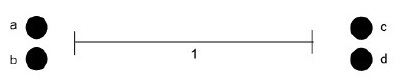
\includegraphics[width=0.6\textwidth]{simple_dataset.jpg}
  \caption{A simple data set.} 
  \label{fig:f1}
\end{figure}

As an example, consider forming the affinity matrix for the dataset in Figure \ref{fig:f1} using Equation \ref{eq:affinity} with $\Theta=1$. Then we get the affinity matrix in Figure \ref{fig:f2}.
\begin{figure}[ht]
  \centering
  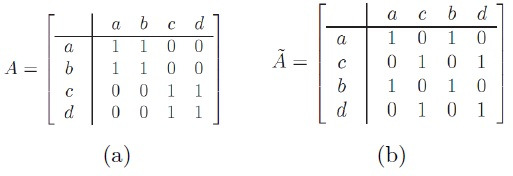
\includegraphics[width=0.6\textwidth]{matrices.jpg}
  \caption{Affinity matrices of Figure \ref{fig:f1} with $\Theta=1$.} 
  \label{fig:f2}
\end{figure}

Now for this particular example, the clusters $\{a, b\}$ and $\{c, d\}$ show up as nonzero blocks in the affinity matrix. This is artificial since we could have constructed the matrix $A$ using an ordering of $\{a, b, c, d\}$. For example, another possible affinity matrix for $A$ could have been as in Figure \ref{fig:f2}(b).

The key insight here is that the eigenvectors of matrices $A$ and $\tilde{A}$ have the same entries (just permuted). The eigenvectors with nonzero eigenvalues of $A$ are $\ve_{1}=(1, 1, 0, 0)^\top$ and $\ve_{2}=(0, 0, 1, 1)^\top$. And the nonzero eigenvectors of $\tilde{A}$ are: $\ve_{1}=(1, 0, 1, 0)^\top$ and $\ve_{2}=(0, 1, 0, 1)^\top$. Spectral clustering embeds the original data points into a new space by using the coordinates of these eigenvectors. Specifically, it maps the point $\vx_{i}$ to the point $\ve_{1}(i), \ve_{2}(i),\dots, \ve_{k}(i)$ where $\ve_{1},\ve_{2},\dots, \ve_{k}$ are the top $k$ eigenvectors of $A$ corresponding to the biggest eigenvalues. We refer to this mapping as the spectral embedding.

\emph{Hint}: This is different from what you learned in class. With the Graph Laplacian $L$, we are trying to find its eigenvectors corresponding to the smallest eigenvalues. What you should notice here is that the matrix $A$ is not Graph Laplacian, this leads to different algorithms. You can analyze the underlying meaning of this approach as what we did in the class.

In this problem, we will analyze the operation of one of the variants of spectral clustering methods on a simple data set shown in Figure \ref{fig:f3}:
 \begin{figure}[ht]
  \centering
  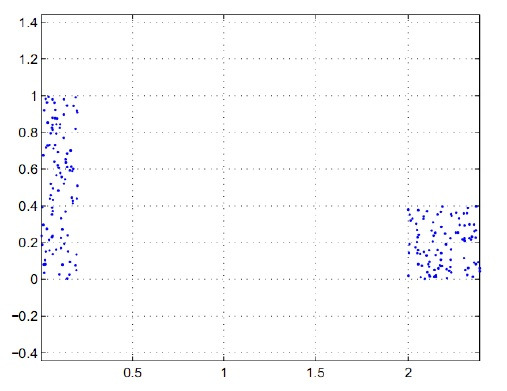
\includegraphics[width=0.6\textwidth]{rec_dataset.jpg}
  \caption{Dataset with rectangles} 
  \label{fig:f3}
\end{figure}

3.1 For the data set in the above figure, assume that the first cluster has $m_{1}$ points and the second one has $m_{2}$ points. If we use Equation \ref{eq:affinity} to compute the corresponding affinity matrix $A$, what $\Theta$ value would you choose and why?

解: 记图 \ref{fig:f3} 中左侧数据为第 1 堆 (cluster), 右侧数据为第 2 堆. 记第 1 堆数据之间的最大距离为 $d_1$, 第 1 堆数据与第 2 堆数据之间的最短距离为 $d_2$. 为使每堆数据之内的相似性度量为 1 而两堆数据之间的相似性度量为 0, 则需选择
\begin{equation}
  \Theta\in(d_1,d_2]
\end{equation}

根据图中具体数据可知, 选择 $\Theta=1.5$ 可以满足上述要求.

3.2 The second step is to compute first $k$ dominant eigenvectors of the affinity matrix, where $k$ is the number of clusters we want to have. For the data set in Figure \ref{fig:f3} and the affinity matrix defined by Equation \ref{eq:affinity}, is there a value of $\Theta$ for which you can analytically compute the first two eigenvalues and eigenvectors? If not, explain why not. If yes, compute and write these eigenvalues and eigenvectors down. What are the other eigenvalues? Explain briefly.

解: 存在, 取 3.1 中 $\Theta=1.5$ 即可解析计算相似 (affinity) 矩阵 $A$ 的前两个特征值与特征向量. 

首先通过调整顺序可写出 $A$ 为
\begin{equation}
  A=\begin{bmatrix}
    \bm{1}_{m_1\times m_1} & \bm{0}_{m_1\times m_2} \\
    \bm{0}_{m_2\times m_1} & \bm{1}_{m_2\times m_2} \\
    \end{bmatrix}
\end{equation}

易知其前两个特征值为 $m_1$ 与 $m_2$, 对应的特征向量分别为
\begin{equation}
  \ve_1=\begin{bmatrix}
    \bm{1}_{m_1\times1}\\
    \bm{0}_{m_2\times1}
  \end{bmatrix},\quad
  \ve_2=\begin{bmatrix}
    \bm{0}_{m_1\times1}\\
    \bm{1}_{m_2\times1}
  \end{bmatrix}
\end{equation}

由于矩阵 $A$ 的秩 $\rank(A)=2$, 则其他特征值均为 0.

3.3 We can now compute the spectral embedding of the data points using the $k$ top eigenvectors. For the data set in Figure \ref{fig:f3}, write down your best guess for the coordinates of the $k=2$ cluster centers using the $\Theta$ that you picked in the first part.

解: 根据 $\ve_1$ 与 $\ve_2$ 可知, 两堆的聚类中心分别为
\begin{equation}
  \vc_1=\begin{bmatrix}
    1\\0
  \end{bmatrix},\quad
  \vc_2=\begin{bmatrix}
    0\\1
  \end{bmatrix}
\end{equation}

\section*{Programming: K-means, hierarchical clustering and spectral clustering}

Test the clustering algorithms K-means, hierarchical clustering and spectral clustering with different parameters on \href{http://yann.lecun.com/exdb/mnist/}{MNIST dataset} or subsets of it when the scale is too large for the algorithm involved.

To compare the effectiveness of different clustering methods, \emph{Normalized mutual information} (NMI) are widely used as a measurement. NMI is defined as following:
\begin{equation}
  \text{NMI} = \frac{\displaystyle\sum_{s=1}^{K}\sum_{t=1}^{K}n_{s,t}\log\left(\frac{nn_{s,t}}{n_{s}n_{t}}\right)}{\displaystyle\sqrt{\left(\sum_{s=1}^Kn_{s}\log\frac{n_{s}}{n}\right)\left(\sum_{t=1}^Kn_{t}\log\frac{n_{t}}{n}\right)}}.
\end{equation}

Where $n$ is the number of data points, $n_{s}$ and $n_{t}$ denote the numbers of the data in class $s$ and class $t$, $n_{s,t}$ denotes the number of data points in both class $s$ and class $t$. For more details and other measurements, google ``evaluation of clustering''.

4.1 Give a brief analysis of time complexity of each algorithm mentioned above (of standard implementation). Estimate how many samples each algorithm can manage with a reasonable time cost.

(Optional) Can you verify your estimations with experiments? Can you speed it up further?

解: 记 $k$ 为分类数, $n$ 为点数, $T$ 为算法循环次数, 则 K-means 算法的复杂度为 $O(knT)$. 分级聚类算法计算两类距离复杂度 $O(n^2)$, 总共计算 $n$ 次, 所以分级聚类算法的复杂度为 $O(n^3)$. 谱聚类算法计算相似度矩阵的复杂度为 $O(n^2)$, 计算特征值与特征向量的复杂度为 $O(n^3)$, 所以谱聚类算法的复杂度为 $O(n^3)$.

以 CPU 主频为 3GHz 来估算, 若需要 1s 之内计算完成, 则最多计算样本数大约为:

(a) K-means: $3\times10^9$

(b) 分级聚类: $\sqrt[3]{3}\times10^3$

(c) 谱聚类: $\sqrt[3]{3}\times10^3$

4.2 Consider each data set, and use the true number of classes as the number of clusters.

(1) With K-means, will the initial partition affect the clustering results? How can you solve this problem? And do $J_{e}$ and NMI match? Show your experiment results.

解: 选择样本数量 $n=3000$, 分别使用 k-means++ \cite{kmeans}, 随机初始化与聚类中心重合初始化三种初始化方法进行 K-means 聚类, 其结果如表 \ref{tab:kmeans_initial} 所示.

\begin{table}[htbp]
  \centering
  \caption{K-means 聚类结果}
  \label{tab:kmeans_initial}
  \begin{tabular}{rcc}
    \toprule
    methods & $J_e\times10^{9}$ & NMI \\
    \midrule
    k-means++ & 7.527918 & 0.495957 \\
    random & 7.514934 & 0.503458 \\ 
    coincide & 7.700415 & 0.473963 \\
    \bottomrule
  \end{tabular}
\end{table}

由表 \ref{tab:kmeans_initial} 可知, 三种初始化方法对聚类结果有影响, 但是影响并不是很大. 实际上, K-means 可能会受到初始化影响而陷入局部极小, 对此我们一般可以采用多次随机初始化, 然后取效果最好的结果. 由表 \ref{tab:kmeans_initial} 也可看出当样本数量相同时, $J_e$ 越小则 NMI 越大, 聚类效果越好. 但是当样本数量发生变化时, $J_e$ 与 NMI 的变化情况则会有所不同.

为了测试 $J_e$ 与 NMI 关于样本数量的变化关系, 选择样本数量 $n=[100,200,\dots,3000]$, 使用 k-means++ 初始化方法得到 K-means 聚类结果 $J_e$ 如图 \ref{fig:kmeans_innertia_pp} 所示, NMI 如图 \ref{fig:kmeans_nmi_pp} 所示.

\begin{figure}[htbp]
  \centering
  \begin{minipage}[t]{0.48\textwidth}
    \centering
    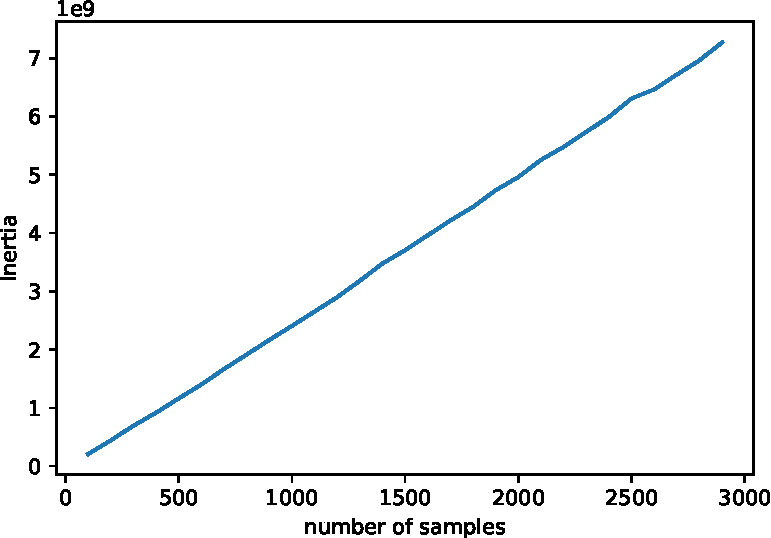
\includegraphics[width=8cm]{kmeans_innertia_pp.pdf}
    \caption{K-means 算法 k-means++ 初始化 $J_e$ 与样本数量变化关系}
    \label{fig:kmeans_innertia_pp}
  \end{minipage}
  \begin{minipage}[t]{0.48\textwidth}
    \centering
    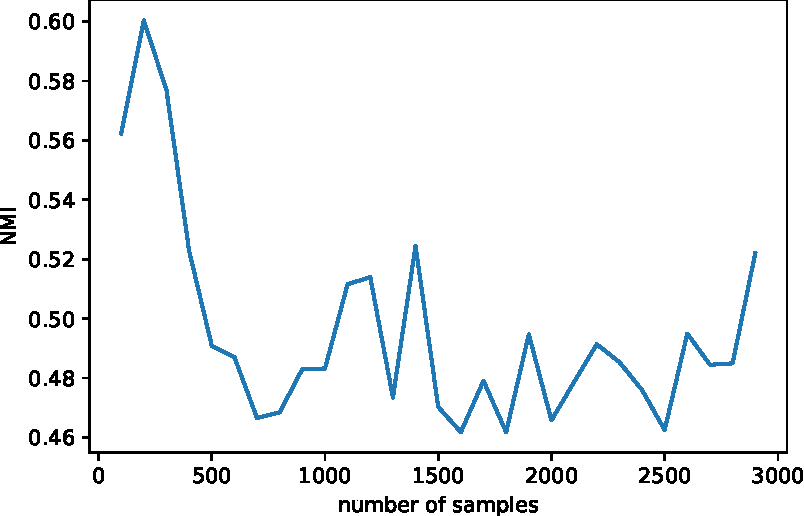
\includegraphics[width=8cm]{kmeans_nmi_pp.pdf}
    \caption{K-means 算法 k-means++ 初始化 NMI 与样本数量变化关系}
    \label{fig:kmeans_nmi_pp}
  \end{minipage}
\end{figure}

使用随机初始化方法得到 K-means 聚类结果 $J_e$ 如图 \ref{fig:kmeans_innertia}  所示, NMI 如图 \ref{fig:kmeans_nmi} 所示.

\begin{figure}[htbp]
  \centering
  \begin{minipage}[t]{0.48\textwidth}
    \centering
    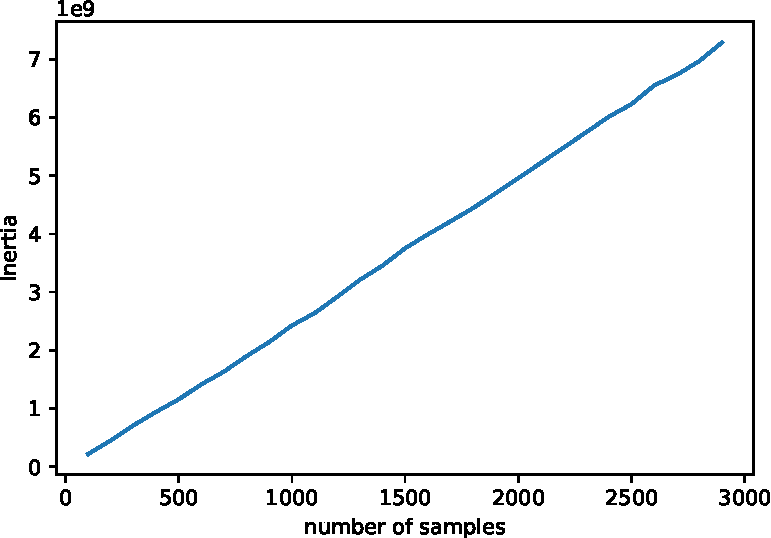
\includegraphics[width=8cm]{kmeans_innertia.pdf}
    \caption{K-means 算法随机初始化 $J_e$ 与样本数量变化关系}
    \label{fig:kmeans_innertia}
  \end{minipage}
  \begin{minipage}[t]{0.48\textwidth}
    \centering
    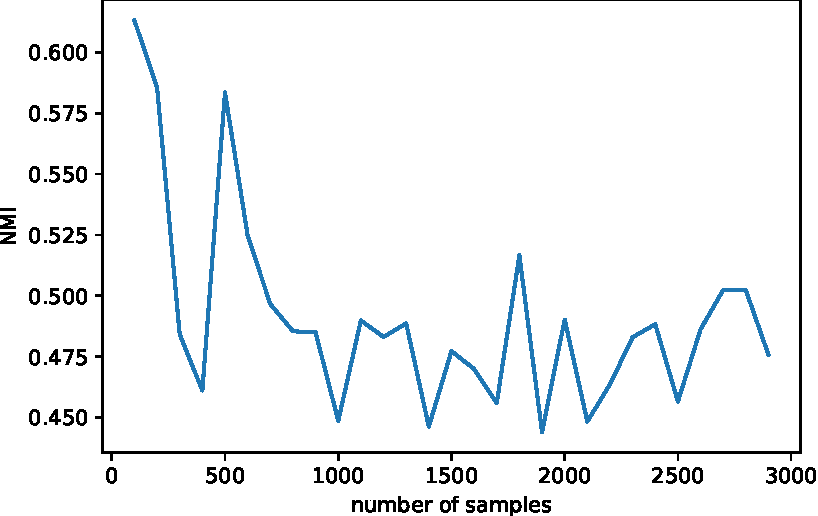
\includegraphics[width=8cm]{kmeans_nmi.pdf}
    \caption{K-means 算法随机初始化 NMI 与样本数量变化关系}
    \label{fig:kmeans_nmi}
  \end{minipage}
\end{figure}

使用聚类中心重合初始化方法得到 K-means 聚类结果 $J_e$ 如图 \ref{fig:kmeans_innertia_coincide} 所示, NMI 如图 \ref{fig:kmeans_nmi_coincide} 所示.

\begin{figure}[htbp]
  \centering
  \begin{minipage}[t]{0.48\textwidth}
    \centering
    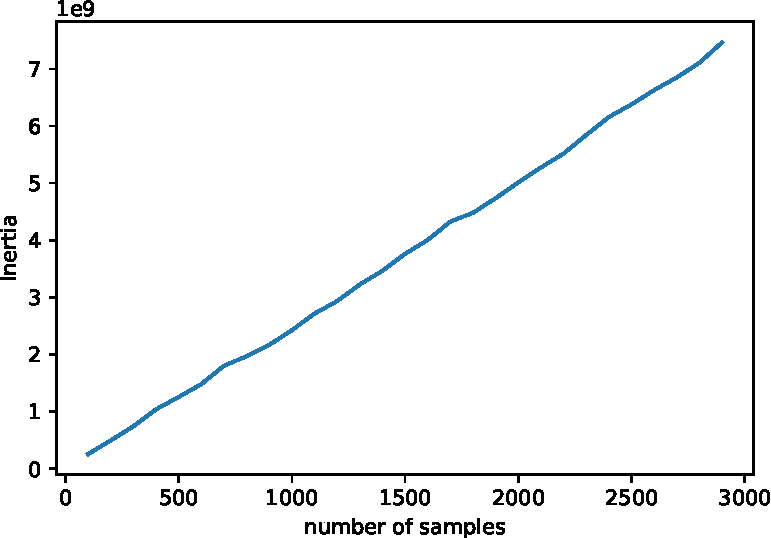
\includegraphics[width=8cm]{kmeans_innertia_coincide.pdf}
    \caption{K-means 算法中心重合初始化 $J_e$ 与样本数量变化关系}
    \label{fig:kmeans_innertia_coincide}
  \end{minipage}
  \begin{minipage}[t]{0.48\textwidth}
    \centering
    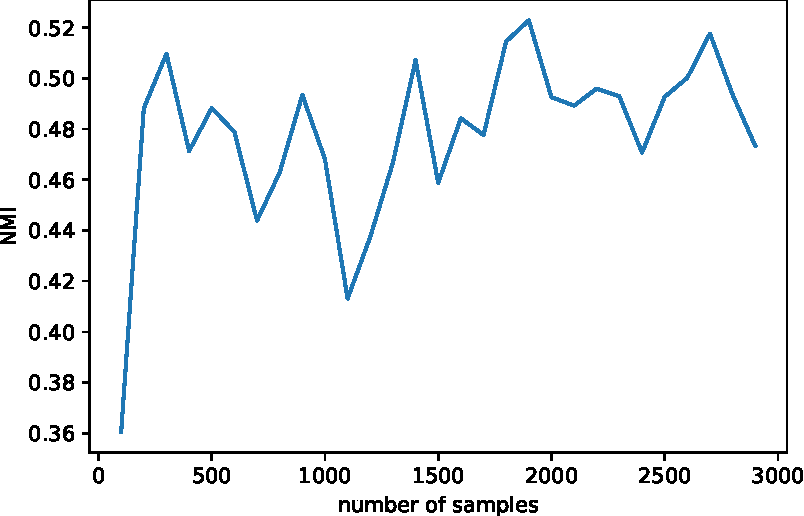
\includegraphics[width=8cm]{kmeans_nmi_coincide.pdf}
    \caption{K-means 算法中心重合初始化 NMI 与样本数量变化关系}
    \label{fig:kmeans_nmi_coincide}
  \end{minipage}
\end{figure}

由此 6 幅对比图可知, 随着样本数量的增长, $J_e$ 单调增加, 但是 NMI 呈现震荡变化, 因此若样本数量发生变化, 则 $J_e$ 与 NMI 的结果不一定匹配 (match).

(2) When hierarchical clustering is adopted, the choice of linkage method depends on the problem. Give an analysis of linkage method's effects with experiments, and which is better in the sense of NMI?

As introduced in the class, some of the most common metrics of distance between two clusters $\{x_{1},\dots, x_{m}\}$ and $\{y_{1},\dots, y_{p}\}$ are:
\begin{itemize}
  \item \emph{Single linkage:} Distance between clusters is the \emph{minimum} distance between any pair of points from the two clusters, i.e.,
  \begin{equation}
    \min_{i, j}\|x_{i}-y_{j}\|
  \end{equation}

  \item \emph{Complete linkage:} Distance between clusters is the \emph{maximum} distance between any pair of points from two clusters, i.e.,
  \begin{equation}
    \max_{i, j}\|x_{i}-y_{j}\|
  \end{equation}

  \item \emph{Average linkage:} Distance between clusters is the \emph{average} distance between all pairs of points from two clusters, i.e.,
  \begin{equation}
    \frac{1}{mp}\sum_{i=1}^{m}\sum_{j=1}^{p}\|x_{i}-y_{j}\|
  \end{equation}
\end{itemize}

解: 为了测试三种不同距离度量的 NMI 关于样本数量的变化关系, 选择样本数量 $n=[100,200,\dots,3000]$, 使用分级聚类方法得到 NMI 如图 \ref{fig:hierarchical_nmi} 所示. 

\begin{figure}[htbp]
  \centering
  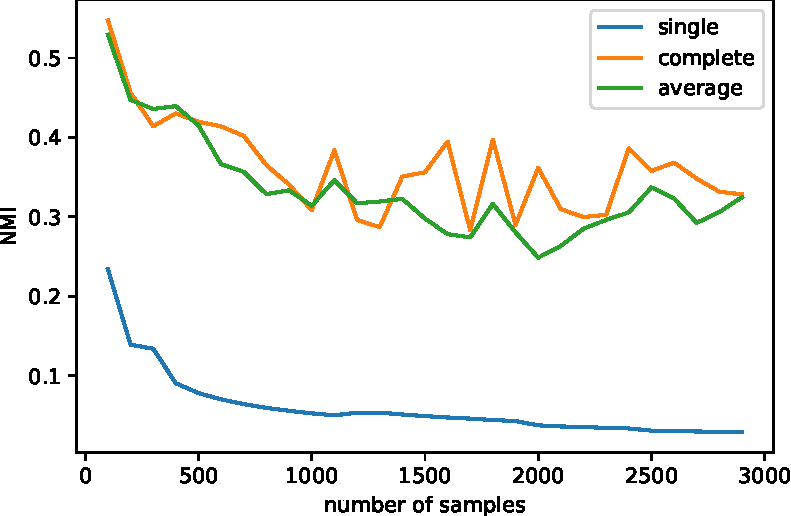
\includegraphics[width=10cm]{hierarchical_nmi.pdf}
  \caption{分级聚类算法不同距离度量 NMI 与样本数量变化关系}
  \label{fig:hierarchical_nmi}
\end{figure}

由图 \ref{fig:hierarchical_nmi} 可知, 最近距离度量的 NMI 普遍低于另外两种度量的 NMI, 最远距离度量的 NMI 与平均距离度量的 NMI 相互交织, 但是大多时候最远距离度量的 NMI 略优于平均距离度量. 这说明 MNIST 数据的各个类别之间距离较近, 可能出现因为边缘距离近导致类别连接的情况. 同时 MNIST 的数据基本围绕在聚类中心各个方向的方差附近, 所以最远距离度量效果较好.

(3) As for spectral clustering, give an experimental analysis of the choice of similarity graph and corresponding parameters. Which one is better?

解: 分别使用高斯核的全连接图和 $k$ 近邻图进行相似矩阵构建, 谱聚类 NMI 结果如表 \ref{tab:spectral_nmi} 所示. 由表 \ref{tab:spectral_nmi} 可知最近邻的效果更好, 选择高斯核的全连接时, 很多点是孤立的因而没有构成一个完全图, 所以聚类效果很差. 而最近邻中 $k=5$ 的效果最好, 若 $k$ 太大, 有可能导致不同类之间的样本连接起来.

\begin{table}[htbp]
  \centering
  \caption{谱聚类全连通图与 $k$ 近邻图实验结果}
  \label{tab:spectral_nmi}
  \begin{tabular}{cc}
    \toprule
    methods & NMI \\
    \midrule
    rbf, $\gamma=1$ &  0.101404 \\
    rbf, $\gamma=2$ &  0.076044 \\
    rbf, $\gamma=4$ &  0.074711 \\
    knn, $k=5$     &  0.614761 \\
    knn, $k=50$    &  0.519622 \\
    knn, $k=100$   &  0.468890 \\
    \bottomrule
  \end{tabular}
\end{table}

4.3 In practice, we may not know the true number of clusters much. Can you give a strategy to identify the cluster number automatically for each algorithm? Show your results.

解: 可以使用轮廓系数 (Silhouette Coefficient) \cite{silhouette} 来进行聚类数量的选择, 其计算公式为
\begin{equation}
  s(i)=\frac{b(i)-a(i)}{\max\{a(i),b(i)\}}
\end{equation}
其中, $b(i)$ 是点 $i$ 到任何其他堆中所有点的最小平均距离, $a(i)$ 是点 $i$ 到其所在堆中其他点的平均距离.

绘出 K-means 的轮廓系数曲线如图 \ref{fig:kmeans_silhouette} 所示, 在轮廓系数曲线中
$k=2$ 时轮廓系数最大, 按照最大轮廓系数选择结果为 $k=2$. 实际上, 我们可以结合一些先验知识, $k=11$ 的轮廓系数仅次于 $k=2$, 与实际的类别数 $k=10$ 更为接近.

\begin{figure}[htbp]
  \centering
  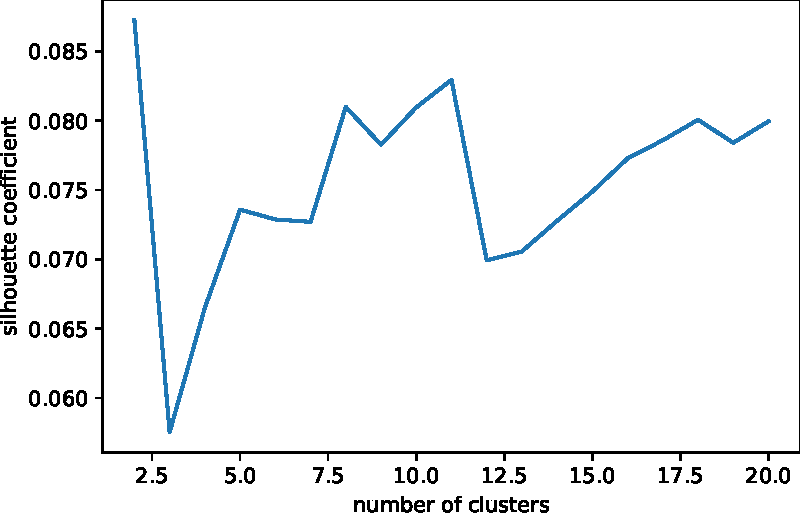
\includegraphics[width=10cm]{kmeans_silhouette.pdf}
  \caption{K-means 算法轮廓系数随聚类类别数变化曲线}
  \label{fig:kmeans_silhouette}
\end{figure}

4.4 According to the above analysis, which method do you prefer? Why?

解: 以上三种聚类方法各有优劣, 聚类方法的选择要根据样本的分布特性和数量综合考虑. 比如若样本点成团状分布或者样本数很大时, 则用 K-means 算法能取得较好效果, 且速度快; 而多级聚类和谱聚类在样本数很大时由于时间复杂度过大而无法使用. 当样本数量较少时, 可以选择基于最近邻图的谱聚类方法, 其聚类的效果较好, 而且不像分级聚类那样受距离度量选择的影响大.

% Reference
\begin{thebibliography}{1}

\bibitem{kmeans}

sklearn.cluster.KMeans, \url{https://scikit-learn.org/stable/modules/generated/sklearn.cluster.KMeans.html#sklearn.cluster.KMeans}.

\bibitem{silhouette}

Rousseeuw, Peter J. ``Silhouettes: a graphical aid to the interpretation and validation of cluster analysis.'' Journal of computational and applied mathematics, 20, 1987: 53-65.

\end{thebibliography}

\end{document}
